\subsection{{\bf RQ1. Comparative Study on Variable Name Prediction.}}
\label{empirical-rq1}

%\begin{table}[t]
%	\caption{RQ1. Comparative Study on Variable Name Prediction.}
%	\begin{center}
%		\small
%		\renewcommand{\arraystretch}{1} 
%		\begin{tabular}{p{2cm}<{\centering}|p{2cm}<{\centering}|p{2cm}<{\centering}}
%			\hline
%		                & Local Variables & All Variables\\
%			\hline
%			JSNice~\cite{JSNice2015}      &                 &         \\
%			JSNaughty~\cite{JSNaughty2017}   &                 &         \\
%                       JSNeat~\cite{icse19}      & 0.64            & 0.66    \\
%			\hline
%			{\tool}     & 0.67            & 0.76    \\
%			\hline
%		\end{tabular}
%		\label{RQ1-result}
%	\end{center}
%\end{table}

\begin{figure}[thbp]
\begin{center}
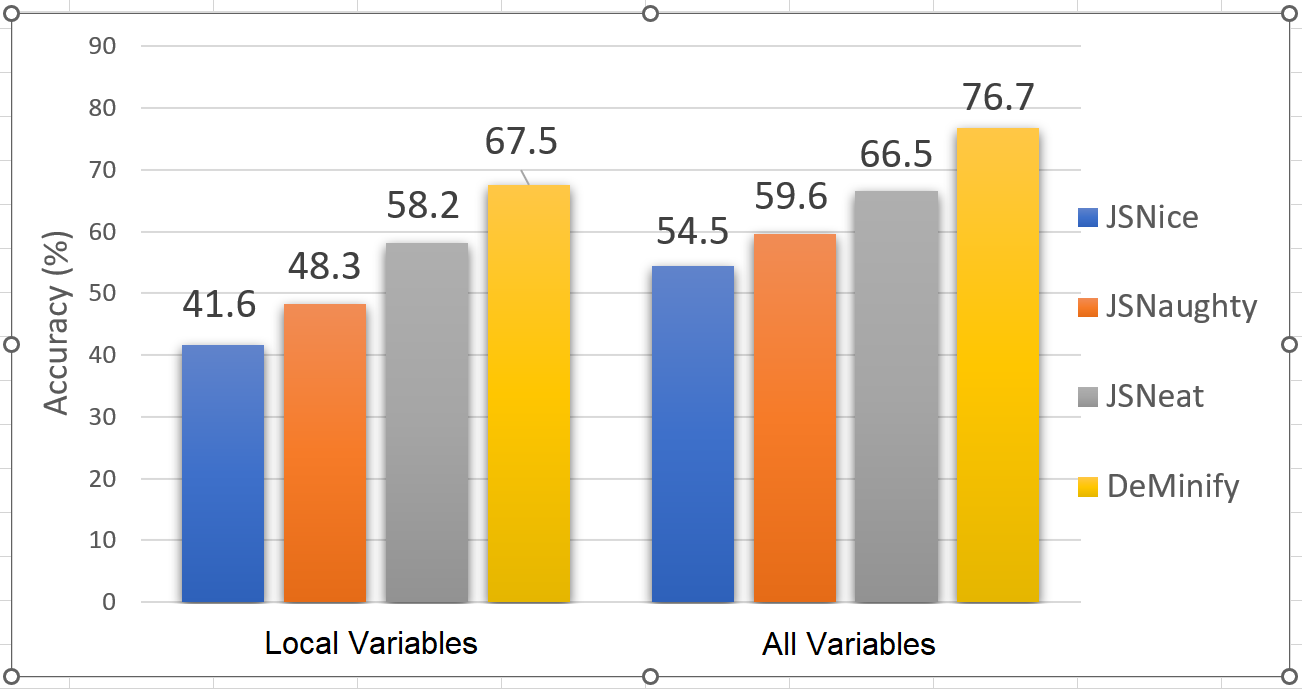
\includegraphics[width=3.2in]{figures/name-prediction-result}
\vspace{-8pt}
\caption{Comparison on Variable Name Prediction}
\label{name-prediction-result}
\end{center}
\end{figure}

In this study, we evaluate {\tool}'s accuracy and compare it with the
state-of-the-art approaches in variable name prediction for minified
code.
%We evaluated {\tool}'s accuracy and compared it with
%JSNice~\cite{JSNice2015} and~JSNaughty \cite{JSNaughty2017}.
%Figure~\ref{comparison_3tools} shows the results.
%for all three tools.
As seen in Figure~\ref{name-prediction-result}, for all variables in
minified code, {\tool} achieves high top-1 accuracy of {\bf 76.7\%}:
in 76.7\% of the cases, it can recover the correct variable names with
a single prediction. The relative improvements in top-1 accuracy for
all variables over JSNice, JSNaughty, and JSNeat are {\bf 40.7\%,
  28.7\%}, and {\bf 15.3\%}, respectively. The absolute improvements
in top-1 accuracy over the state-of-the-art approaches are from
10.2\%--22.2\%.

Considering only local variables, in {\bf 67.5\%} of them, {\tool}
correctly predicts their original names with a single result. The
relative improvements in top-1 accuracy in recovering local variables'
names over JSNice, JSNaughty, and JSNeat are {\bf 62.2\%, 39.8\%}, and
{\bf 15.9\%}, respectively. The absolute improvements in top-1
accuracy over the state-of-the-art approaches are from 9.3\%--25.9\%.

We examined the predicted names from all the baselines. Compared to
JSNeat, an information retrieval approach, we found that it often
failed in the following cases. (1) It has not seen the names before in
the database. {\tool} can generate a new name with its decoder. Due to
explicitly setting of similarity thresholds, it faces two other
issues. (2) The correct name was not returned because the relations
and contexts are not similar enough with pre-defined thresholds.  (3)
if two variables in the same function are assigned with the same name
via the similarity measure, JSNeat cannot decide one, turning to a
random selection. Avoiding feature matching with explicit similarity
threshold, {\tool} with its neural network can implicitly do so
without any similarity threshold.

Compared to JSNaughty~\cite{JSNaughty2017} with statistical machine
translation from minified code to original code, we found that it
relies much on the {\em minified names} in minified code. We examine
the {\em phrase mapping table}, a byproduct of their machine
translation model, which contains the knowledge it learned from
training. We reported that JSNaughty learns {\em inconsistent
  mappings} between the minified names and original ones. That is,
there are several mappings for the same minfied names with different
weights depending on their occurrences in the corpus. For example,
\code{b} $\leftrightarrow$ \code{doc}, \code{b} $\leftrightarrow$
\code{book}, etc. In contrast, {\tool} does not rely on the minified
names themselves, by considering modeling them as the nodes with
missing features (i.e., missing names and types) in the GCNmf
model~\cite{GCNmf}.

{\tool} is similar in spirit to JSNice~\cite{JSNice2015} in which both
formulates the problem as predicting the features/attributes of the
nodes in a graph. The Conditional Random Field in JSNice uses
probabilistic name prediction graph. In comparison, {\tool} leverages
more advanced neural network in GCNmf~\cite{GCNmf} as well as a more
specialized graph with the help of the type prediction model.

%which is not as powerful as the advanced neural network
%GCNmf~\cite{GCNmf}.


%1. On both local variables and all variables, {\tool} performs XXX\%
%better than the baselines.

%2. JSNeat uses information retrieval techniques to find the possible
%variable names based on the training data. {\tool} can perform better
%because sometimes it is hard to find similar variable names with
%similar variable relationships, and sometimes the same variable names
%may have different variable relationships. JSNeat cannot perform well
%in these cases, but {\tool} can still work as designed.

%3. JSNice uses conditional random field models to predict variable
%names based on dependency graphs. {\tool} can outperform {\tool} by
%XX\% because {\tool} uses combine graph from relation graph and
%TDG. The combined graphs contain more detailed information between
%variables compared with dependency graphs.

%4. JSNaughty regards the name prediction problem as the translation
%problem. {\tool} can outperform JSNaughty XX\% because different
%minification tools can provide different minified variable names for
%the same source code, but {\tool} regards the minified variable names
%as missing features in GCNmf. In this case, the minified variable
%names will not influence the performance of {\tool}, but it will
%influence JSNaughty performance.
